\chapter{\label{ch:6-michel}Study of Michel Electrons in \protodune{}} 

\minitoc

%%%%%%%%%%%%%%%%%%%%%%%%%%%%%%%%%%%%%%%%%%%%%%%%%%%%%%%%%%%%%%%%%%%%%%%%%%%%%%%%
% FROM COS
%
% This chapter will cover the primary analysis of this thesis; a study of Michel
% electrons in the ProtoDUNE--SP detector which aims to investigate the agreement
% between data and simulation, and to provide an estimate of the energy scale
% uncertainty and energy scale bias for electrons in the 0--60 MeV range. 
% 
% The work done for this section is ongoing; preliminary work on this topic was
% presented in the report submitted for transfer of status. The rest of the work
% for this section is expected to be completed by the end of October 2019.
% 
% \noindent The work done as of writing for this chapter is as follows:
% \begin{itemize}[noitemsep,nolistsep]
% 	\item Event selection algorithm developed based on clustering of the Michel
% 	like hits discussed in the previous chapter.
% 	\begin{itemize}[noitemsep,nolistsep]
% 		\item Purity of > 98\% and efficiency of 5\% measured in ProtoDUNE--SP 
% 		simulations.
% 	\end{itemize}
% 	\item Two possible energy reconstruction algorithms developed.
% 	\begin{itemize}[noitemsep,nolistsep]
% 		\item Cone algorithm.
% 		\item Semantic segmentation algorithm with U-ResNet CNN architecture.
% 	\end{itemize}
% \end{itemize}
% 
% \noindent The work left to do is as follows:
% \begin{itemize}[noitemsep, nolistsep]
% 	\item Validation of algorithms on the real ProtoDUNE--SP data.
% 	\item Data MC comparison for Michel electron energy spectrum.
% 	\item Energy scale uncertainty and energy scale bias measurements with 
% 	measured Michel electron energy spectrum.
% \end{itemize}
% 
% \noindent An example Michel electron candidate event from the real ProtoDUNE--SP 
% data is given in figure \ref{fig:michel_event}.
% 
% \begin{figure}[h]
% 	\centering
% 	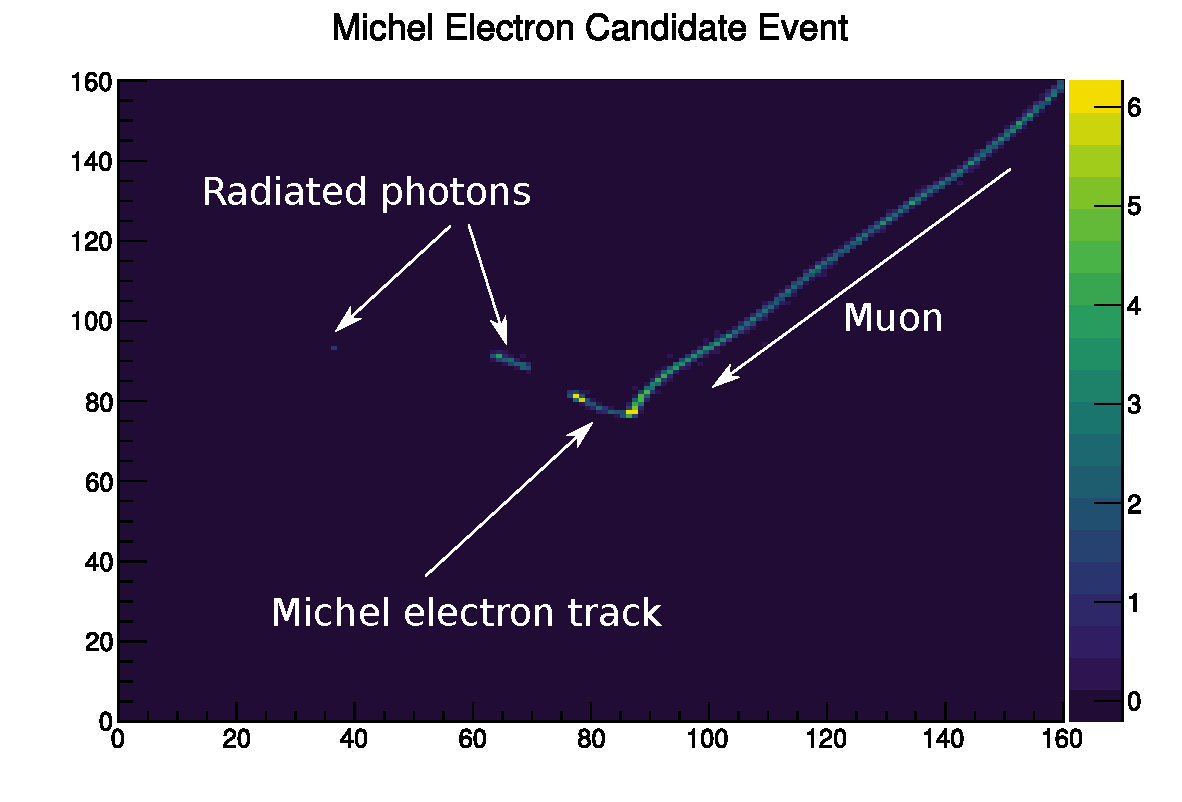
\includegraphics[width=0.7\textwidth]{figures/michel_candidate.pdf}
% 	\caption[Michel electron candidate event from ProtoDUNE--SP data.]{Michel 
% 	electron candidate event from ProtoDUNE--SP data.}
% 	\label{fig:michel_event}
% \end{figure}
%
%%%%%%%%%%%%%%%%%%%%%%%%%%%%%%%%%%%%%%%%%%%%%%%%%%%%%%%%%%%%%%%%%%%%%%%%%%%%%%%%

Studying electrons in the tens of MeV energy range can provide valuable input 
into reconstruction techniques and energy uncertainty for the measurement of
astrophysical neutrinos from supernova bursts. Understanding the response of
LArTPC detectors to electrons in this range will be important for any large
scale LArTPC experiment wishing to study supernova bursts. At these energies
electron interactions have large contributions from both ionisation energy loss
and radiative energy loss and therefore they have a unique signature which is 
neither track--like or shower--like. Low--energy electrons therefore require 
unique reconstruction algorithms to maximise the overall reconstruction 
performance. This chapter will discuss an approach to low--energy electron
reconstruction in LArTPC detectors based on the use of convolutional neural
networks and semantic segmentation. Michel electron events from \protodune{} will
be used to test the performance of this technique and to provide an estimate of
the energy uncertainty of LArTPC detectors for low--energy electrons.

\mccorrect{Chapter outline.}

\section{Michel Electrons in Liquid Argon} \label{ME_LAr}
\begin{mccorrection}
	Michel electrons
	\begin{itemize}
	\item Two types: at rest and captured
	\item Energy spectra
	\end{itemize}
\end{mccorrection}

Michel electrons are produced when a muon decays at rest. This decay gives rise
to a characteristic energy spectrum which has a sharp cut--off at around 50 MeV,
corresponding to half the muon mass. In matter it is also possible for $\mu^-$ 
to be captured on nuclei before they decay, this causes a broadening of the 
Michel electron spectrum for these events. A comparison of the Michel electron 
energy spectrum for free $\mu^+$ and captured $\mu^-$ is given in Fig.
\ref{fig:michel_spec}. The capture process occurs roughly 70\% of the time for
negative muons in liquid argon and therefore in \protodune{} the observed energy
spectrum is a combination of the two processes in roughly equal quantities.

\begin{figure}

	\centering

	\includegraphics[width=\textwidth]{figures/michel_spectra.pdf}

	\caption
	[Michel electron energy spectra in Liquid Argon]
	{Michel electron energy spectra in liquid argon. (a) free muons. (b) muon 
	capture at rest.}

	\label{fig:michel_spec}

\end{figure}

\begin{mccorrection}
	Electron and photon energy loss 
	\begin{itemize}
	\item Ionisation to radiative transition
	\item Event signature
	\item Example event
	\item Photon radiation length
	\item Photon spectrum
	\item Photon multiplicity
	\item Fractional energy loss vs energy
	\end{itemize}
\end{mccorrection}

As discussed in chapter \ref{ch:4-energyloss}, the energy loss for electrons in
liquid argon passes from an ionisation dominated regime to a radiation dominated
regime in the tens of MeV region. The crossover point for this transition occurs
at around 45 MeV, very close to the peak of the Michel electron spectrum. This
leads to a unique signature for Michel electrons in liquid argon detectors, a
short ($\sim$ 5cm) track segment is surrounded by a number of small radiated 
energy deposits. Figure \ref{fig:michel_event} shows an example of a Michel 
electron candidate from \protodune{} data, along with labels of the key 
features.

\begin{figure}
	\centering
	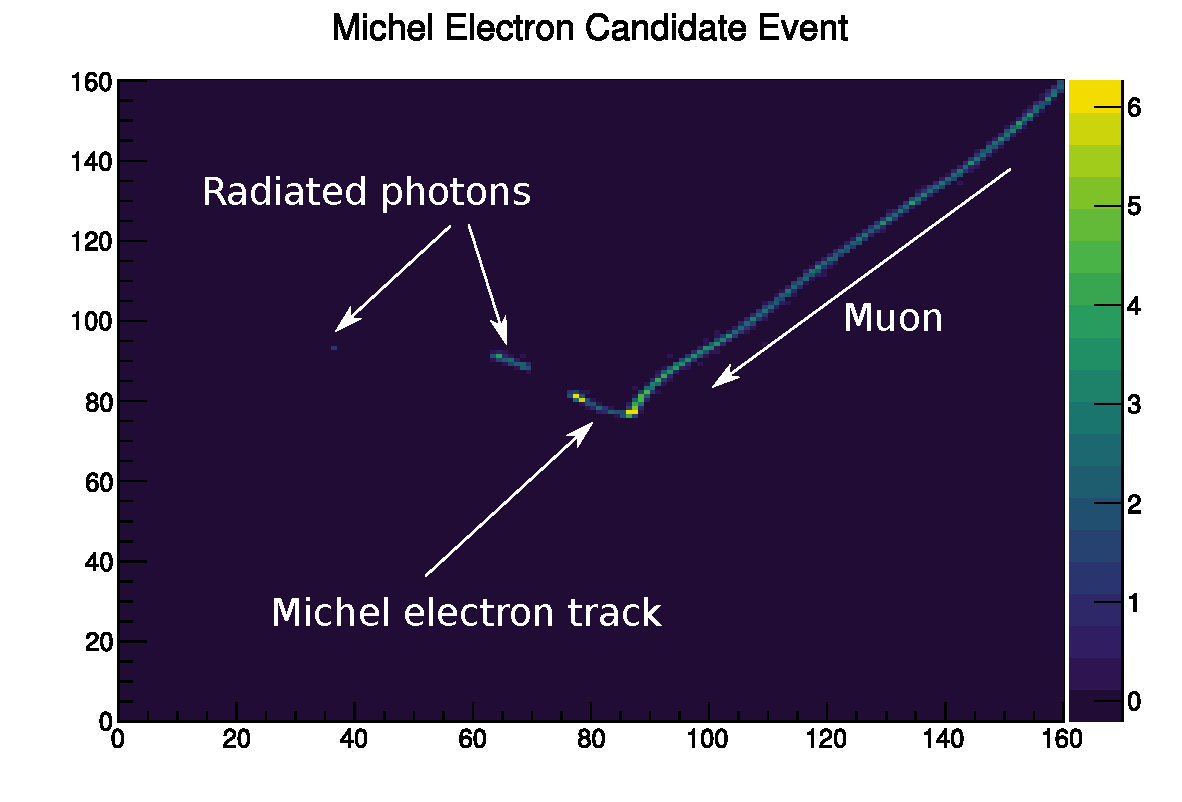
\includegraphics[width=\textwidth]{figures/michel_candidate.pdf}
	\caption
	[Michel electron candidate event from ProtoDUNE--SP data.]
	{Michel electron candidate event from ProtoDUNE--SP data.}
	\label{fig:michel_event}
\end{figure}

One of the main challenges for Michel electron reconstruction in liquid argon is
to successfully associate the radiated energy depositions back to the initial
Michel electron once they have produced ionisation in the detector. Photons have
a radiation length of around 20--30 cm in liquid argon which is many times
larger than the size of the typical track--like part of the event, around 5 cm. 
Fig. \ref{fig:photon_spec} shows the spectrum of radiated photons from Michel 
electron events in \protodune{} simulation alongside the photon multiplicity 
as a function of Michel electron energy. While most of the radiated photons 
only carry a small fraction of the Michel electrons energy, in some cases a 
single radiated photon can carry a significant fraction of the electron 
energy. In addition, around the peak of the Michel electron spectrum ($\sim$
45 MeV) there is a high photon multiplicity and a large spread in the
multiplicity distribution. The combination of these effects leads to a
significant spread in the fraction of radiated energy for Michel electron
events.

\begin{figure}
	% TODO: split into 2 figures
	\centering
	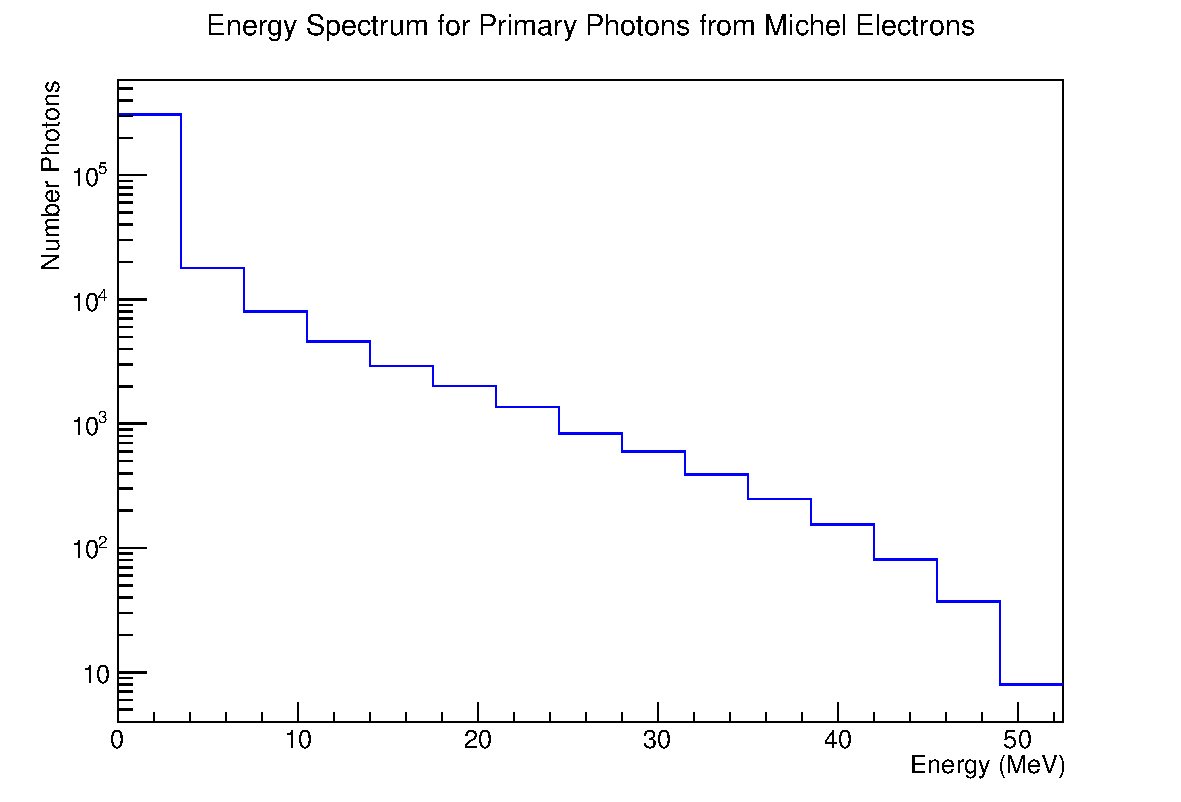
\includegraphics[width=\textwidth]{figures/photon_spec.pdf}
	\newline
	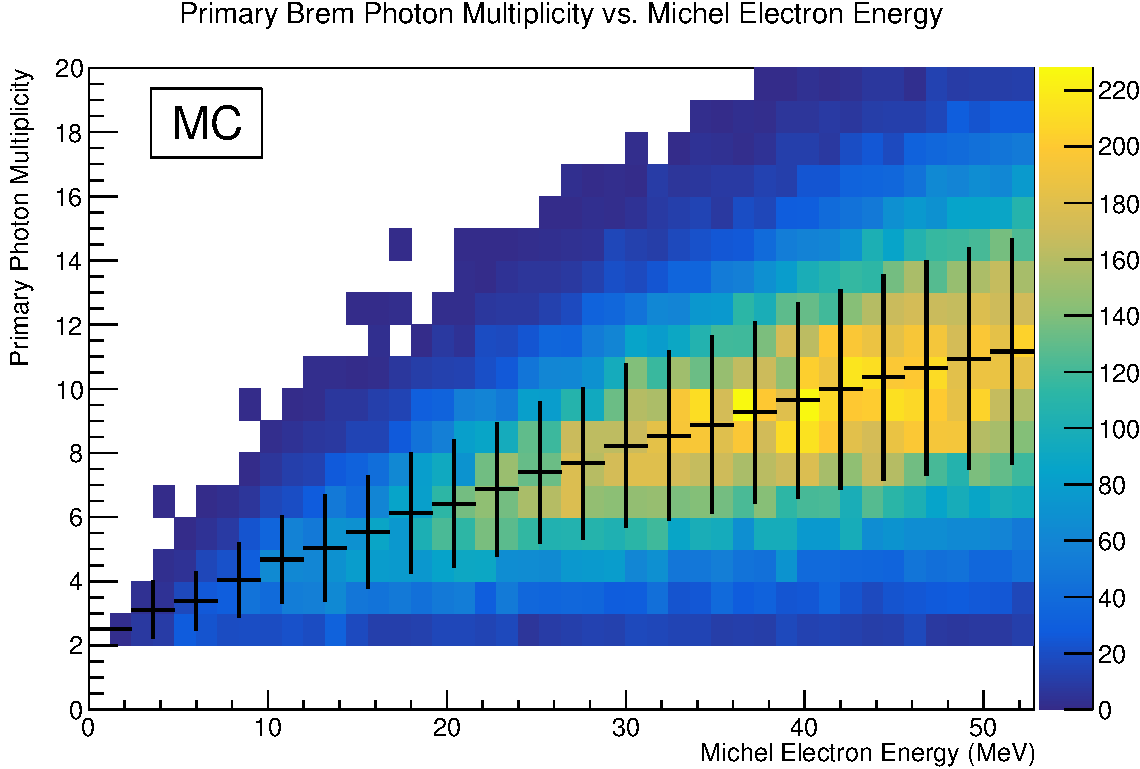
\includegraphics[width=\textwidth]{figures/photon_mult.pdf}
	\caption
	[Energy spectrum and multiplicity of radiated photons from Michel electron 
	events.]
	{Energy spectrum  and multiplicity of radiated photons from Michel electron events in
	\protodune{} simulation. 
	(a) Energy spectrum of radiated photons, log scale. 
	(b) Radiated photon multiplicity vs Michel electron energy. 
	}
	\label{fig:photon_spec}
\end{figure}

\mccorrect{Paragraph + figure on fraction of energy lost to radiation.}

\begin{mccorrection}
	Impact on event geometry and energy reco
	\begin{itemize}
	\item Track only ionisation
	\item Geometry of radiation
	\item 40cm ionisation 
	\item Need to collect radiative photons
	\end{itemize}
\end{mccorrection}

The energy which is lost into radiated photons is only visible once the photons
interact in the argon to produce secondary electrons which then ionise the
argon. These secondary electrons are scattered over large angles and distances
in the detector when compared to the short Michel electron track, the spatial 
distribution of secondary electrons is shown in Fig. \ref{fig:photon_geom}.
\mccorrect{TODO, analysis.}
\begin{figure}
	\centering
	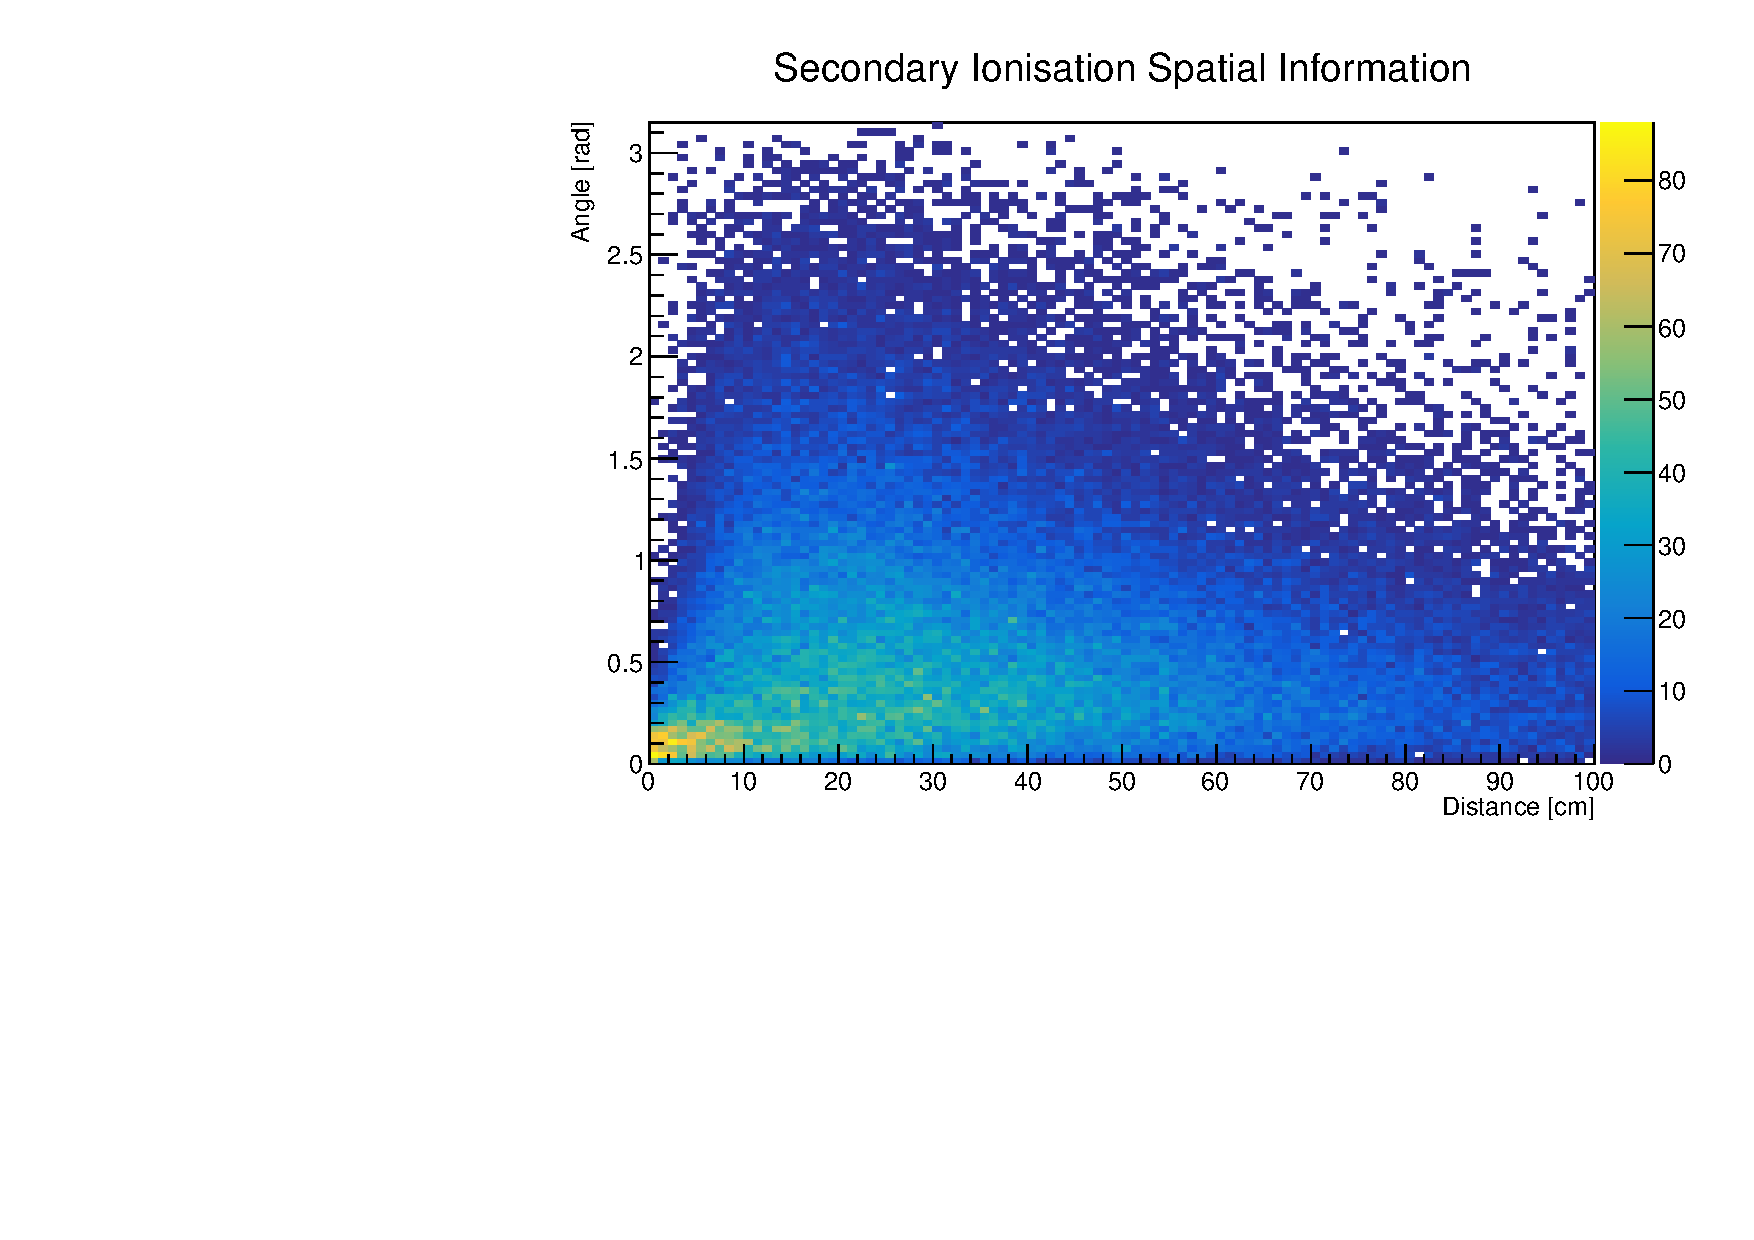
\includegraphics[width=\textwidth]{figures/photon_geom.pdf}
	\caption
	[Spatial distribution of radiated ionisation deposits.]
	{Spatial distribution of radiated ionisation deposits.}
	\label{fig:photon_geom}
\end{figure}

To highlight the impact of the radiated energy deposits we can consider the 
results of perfect energy reconstruction in two cases:
\begin{itemize}
	\item Only considering the Michel electron track.
	\item Considering all ionisation energy within some radius and angle of the 
		Michel electron track.
\end{itemize}
Fig. \ref{fig:michel_track_only} illustrates the considerable increase in energy
collected if radiated energy is considered, the distribution is significantly
narrower and much more energy is recovered when considering the energy deposited
within a cone of height 40cm and angle 30 \textdegree of the Michel electron
vertex. The average energy recovered is increased from \mccorrect{TODO \%} to
\mccorrect{TODO \%} and the spread is reduced from \mccorrect{TODO \%} to
\mccorrect{TODO \%}.
\begin{figure}
	\centering

	\begin{subfigure}{\textwidth}
		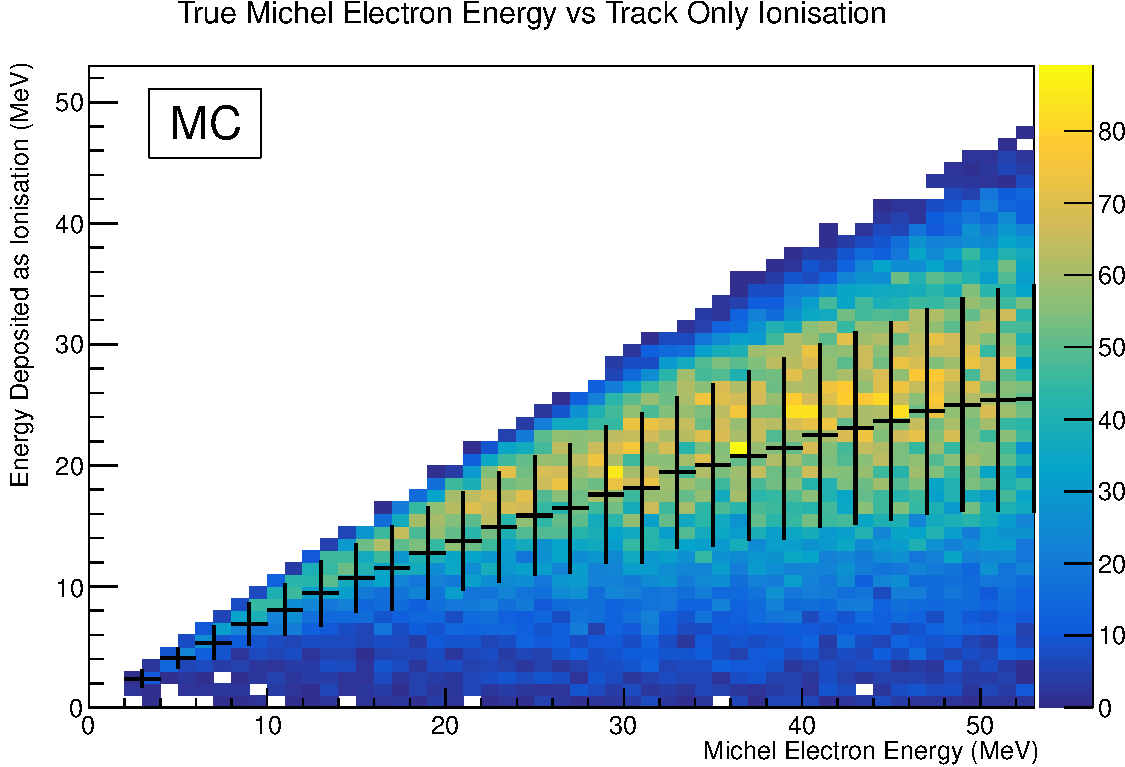
\includegraphics[clip, trim = 0cm 0cm 0cm 1cm, width=0.49\textwidth]{figures/michel_track_only.pdf}
		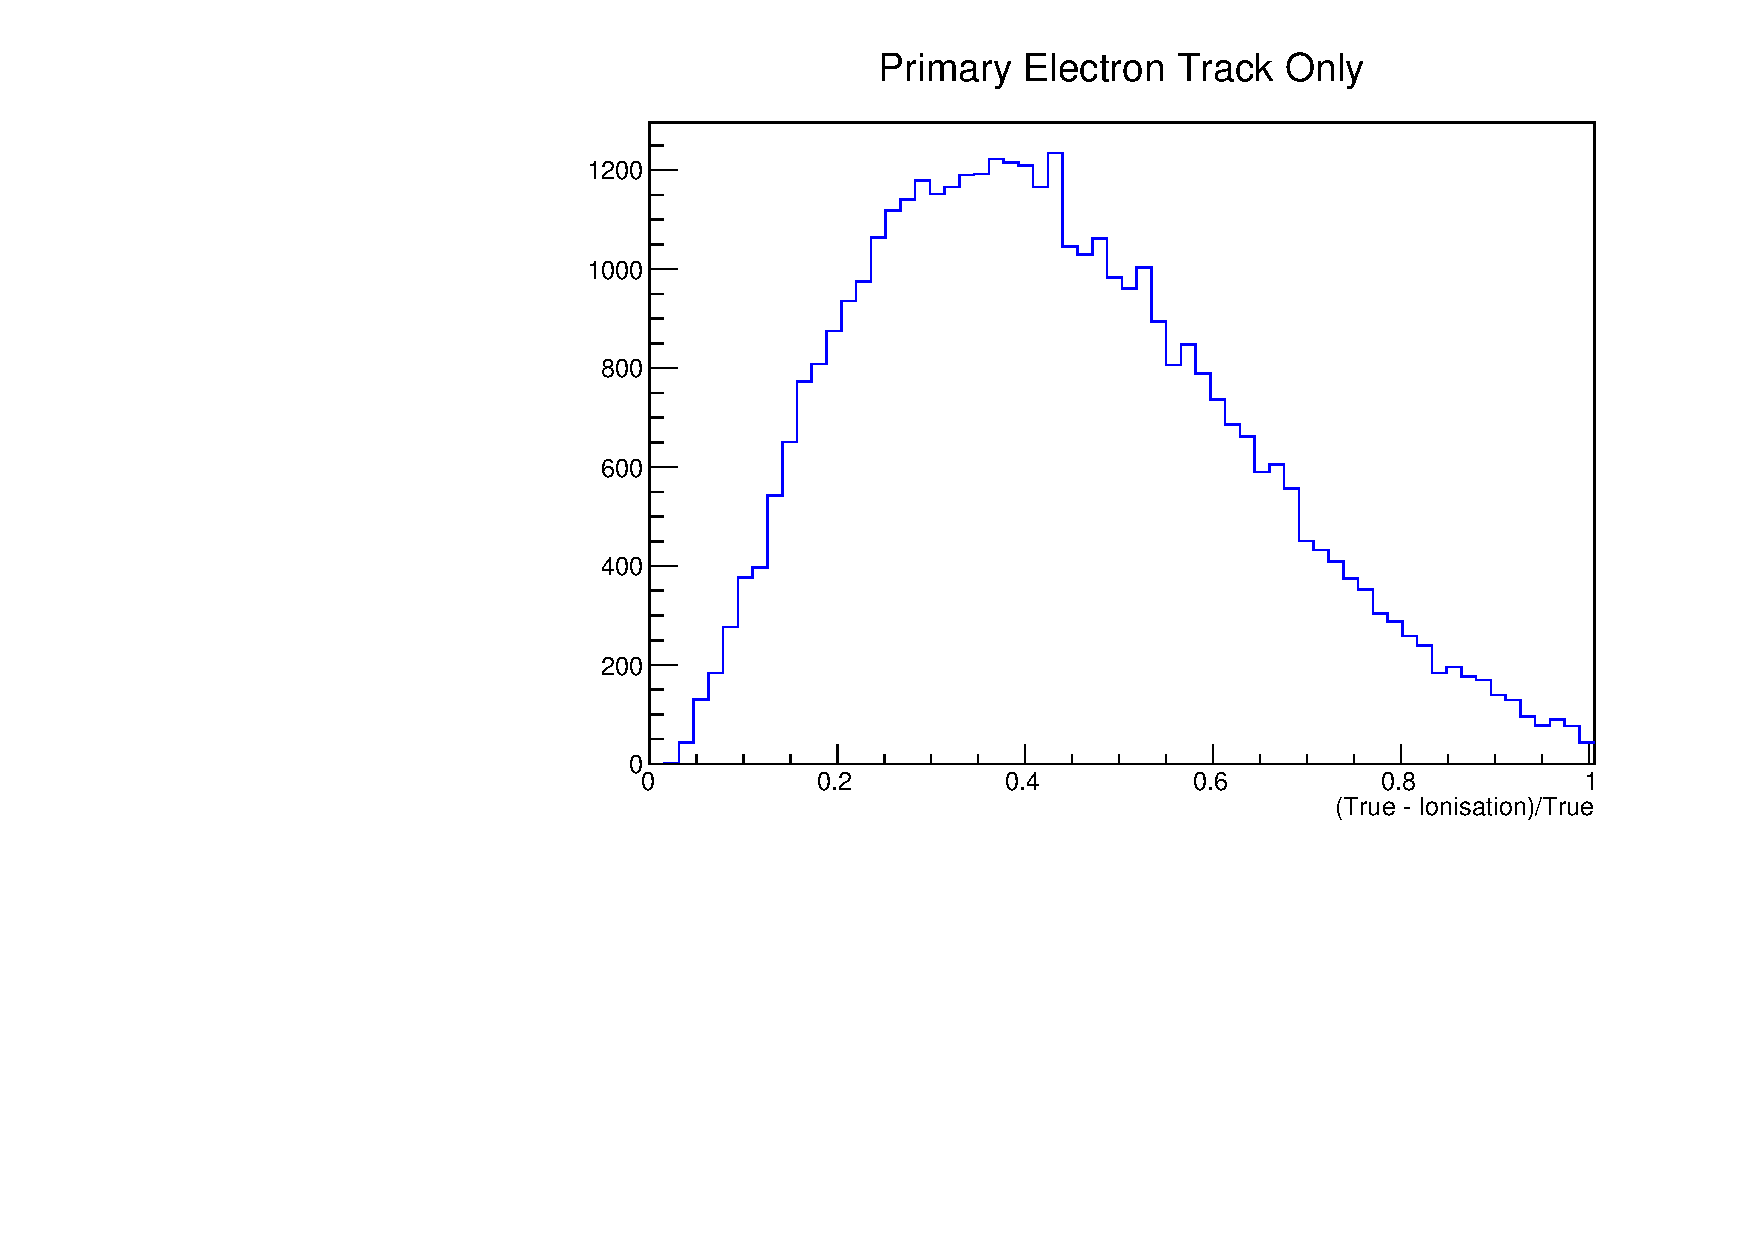
\includegraphics[clip, trim = 0cm 0cm 0cm 1cm, width=0.49\textwidth]{figures/track_frac.pdf}
	\end{subfigure}
	\begin{subfigure}{\textwidth}
		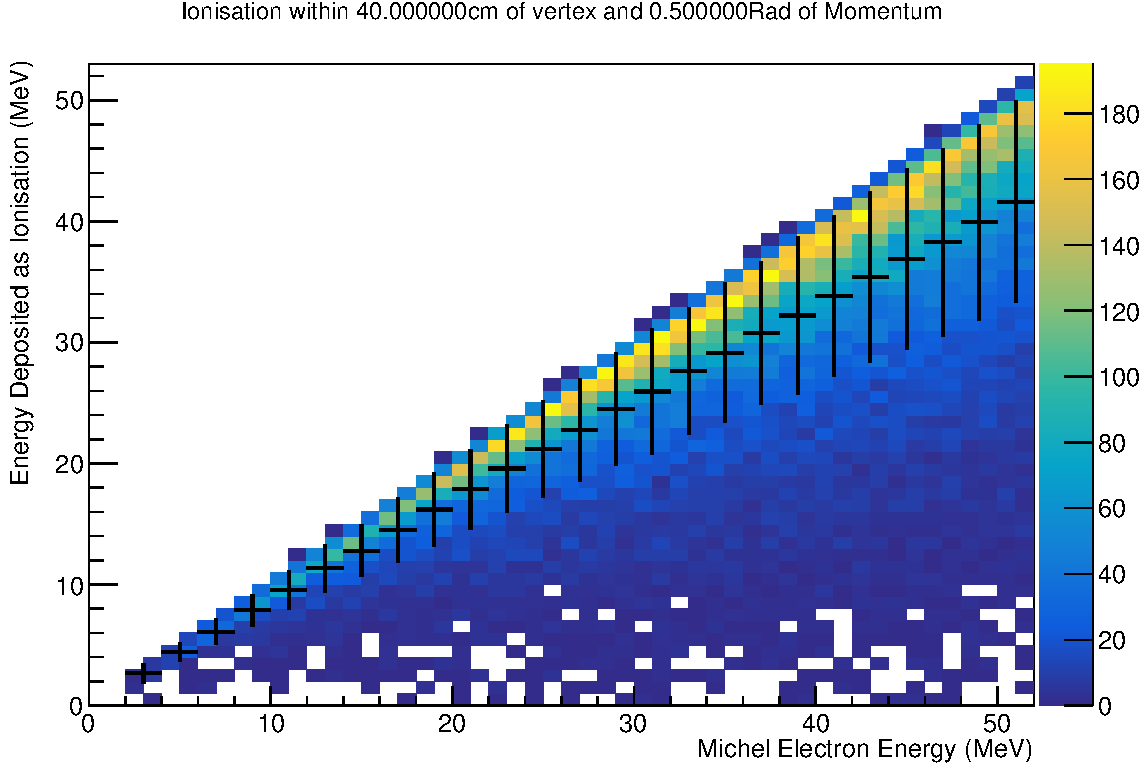
\includegraphics[clip, trim = 0cm 0cm 0cm 1cm, width=0.49\textwidth]{figures/cone_reco.pdf}
		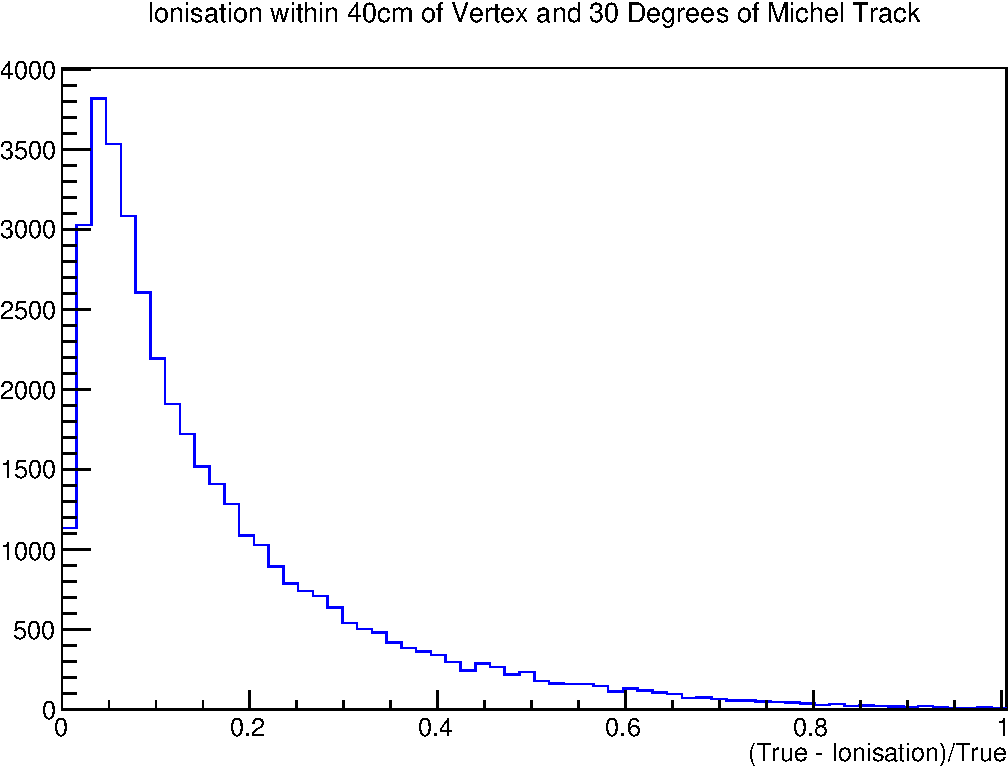
\includegraphics[clip, trim = 0cm 0cm 0cm 1cm, width=0.49\textwidth]{figures/cone_frac.pdf}
	\end{subfigure}

	\caption
	[Comparison of track--only ionisation and ionisation within a collection cone.]
	{Comparison of track--only ionisation and ionisation within a collection cone.}

	\label{fig:michel_track_only}

\end{figure}

\mccorrect{TODO, figure and paragraph for energy fraction vs radius.}
\begin{figure}
	\centering
	% TODO
	\includegraphics[width=\textwidth]{figures/frac_v_radius.pdf}
	\caption
	[Fraction of Michel electron energy collected vs collection radius.]
	{Fraction of Michel electron energy collected vs collection radius.}
	\label{fig:frac_v_radius}
\end{figure}

The MC study presented here highlights the importance of radiated energy
deposits in Michel electron and other low--energy electron events. Based on
these results it is clear that to minimise energy uncertainties for these events
it is important to maximise the amount of energy collected from radiated 
photons. The rest of this chapter will discuss an algorithm which was developed 
to tackle this problem, and it's application on Michel electron events in 
\protodune{} data.

\section{Michel Electron Event Selection} \label{ME_ES}
\begin{mccorrection}
	\begin{itemize}
	\item Michel hit tagging CNN
	\item Hit tagging + clustering explanation
	\item Algorithm performance: purity and efficiency
	\item CNN distributions
	\item Data v MC event selection distributions
	\end{itemize}
\end{mccorrection}

In order to select Michel electrons in \protodune{} data, an event selection
algorithm was developed based on combining the results from the hit tagging CNN 
from the previous chapter with clustering performed by the main \protodune{} 
reconstruction framework, Pandora. 

The event selection algorithm proceeds in the following steps:
\begin{enumerate}
	\item Start with all primary tracks from Pandora.
	\item Define a set of Michel electron candidates from the list of all
		daughters of the track.
	\item Find the best Michel electron candidate from the list of Michel electron
		candidates.
	\item Select events where the best Michel electron candidate passes the event
		selection cuts.
\end{enumerate}

In the first step the initial sample of muon candidates is defined. All tracks
from the Pandora reconstruction chain which have been labelled as primary tracks
are considered.

The second step defines a set of Michel electron candidates for each track in
the sample. A Michel electron candidate is any daughter of the primary Pandora
track which satisfies the following conditions:
\begin{itemize}
	\item Starts within 5 cm of the primary track endpoint.
	\item Contains a minimum of 5 hits on the collection plane.
\end{itemize}

In the third step the Michel electron candidates are analysed in order to define
the best Michel electron candidate for each track. The best Michel electron
candidate is the Michel electron candidate with the largest fraction of
Michel--like hits based on the output of the Michel electron score from the CNN
with a threshold of 0.9. In the case of a tie the Michel electron candidate with
the most hits is chosen.

The fourth step is the final decision, if the best Michel electron candidate is
made up of more than 80 \% of Michel--like hits then it is selected as a
Michel electron candidate.

Based on this algorithm Michel electron events are selected with over
\mccorrect{TODO \%} purity and \mccorrect{TODO \%} efficiency in \protodune{}
simulation. Figure \ref{fig:michel_like_frac} shows a comparison of the fraction of Michel--like
hits for the best Michel electron candidate in \protodune{} data and simulation.
\mccorrect{TODO, analysis and figure}.
\begin{figure}
	\centering
	% TODO
	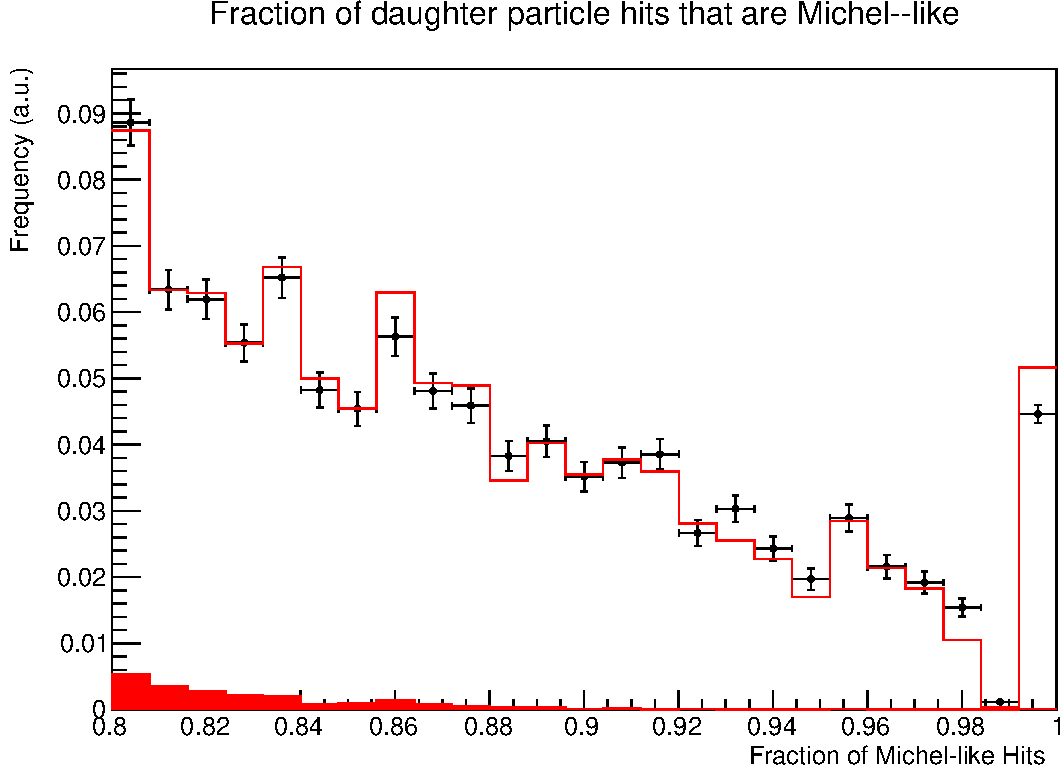
\includegraphics[width=\textwidth]{figures/michel_like_frac.pdf}
	\caption
	[Fraction of Michel--like hits in the best Michel electron candidate.]
	{Fraction of Michel--like hits in the best Michel electron candidate.}
	\label{fig:michel_like_frac}
\end{figure}

\mccorrect{TODO: Event selection distributions.}

\section{Michel Electron Energy Reconstruction} \label{ME_R} 
\begin{mccorrection}
	\begin{itemize} 
	\item U-Nets and semantic segmentation
	\item Algorithm outline
	\item Details of my U-Net
	\item Architecture plot
	\item Map examples
	\item Data v MC score distribution
	\item Reco spectrum
	\item NHits
	\item Energy per hit
	\item Reco geometry variables
	\end{itemize}
\end{mccorrection}

\section{Energy Uncertainty for Michel Electrons} \label{ME_EU}
\begin{mccorrection}
	\begin{itemize}
	\item Reco energy scaling
	\item Uncertainty vs energy
	\item Differences in dune far detector
	\end{itemize}
\end{mccorrection}
